\documentclass{article}

\usepackage{hyperref}
\hypersetup{
    colorlinks=true,
    linkcolor=blue,
    filecolor=magenta,      
    urlcolor=cyan,
}

\usepackage{fancyhdr}
\usepackage{extramarks}
\usepackage{amsmath}
\usepackage{amsthm}
\usepackage{amsfonts}
\usepackage{tikz}
\usepackage[plain]{algorithm}
\usepackage{algpseudocode}

\usepackage{listings}
\usepackage{color} 
\definecolor{mygreen}{RGB}{28,172,0} 
\definecolor{mylilas}{RGB}{170,55,241}

\lstset{
    basicstyle=\scriptsize\sffamily\color{black},
    frame=single,
    numbers=left,
    showspaces=false,
    showstringspaces=false,
    tabsize=1
}
\lstset{language=Matlab,%
    %basicstyle=\color{red},
    breaklines=true,%
    morekeywords={matlab2tikz},
    keywordstyle=\color{blue},%
    morekeywords=[2]{1}, keywordstyle=[2]{\color{black}},
    identifierstyle=\color{black},%
    stringstyle=\color{mylilas},
    commentstyle=\color{mygreen},%
    showstringspaces=false,%without this there will be a symbol in the places where there is a space
    numbers=left,%
    numberstyle={\tiny \color{black}},% size of the numbers
    numbersep=9pt, % this defines how far the numbers are from the text
    emph=[1]{for,end,break},emphstyle=[1]\color{red}, %some words to emphasise
    %emph=[2]{word1,word2}, emphstyle=[2]{style},    
}

\topmargin=-0.45in
\evensidemargin=0in
\oddsidemargin=0in
\textwidth=6.5in
\textheight=9.0in
\headsep=0.25in


\linespread{1.1}

\pagestyle{fancy}
\fancyhf{}
\lhead{\hmwkAuthorName}
\chead{\hmwkClass: \hmwkTitle}
\rhead{\leftmark}
\lfoot{\lastxmark}
\cfoot{\thepage}

\renewcommand\headrulewidth{0.4pt}
\renewcommand\footrulewidth{0.4pt}

\setlength\parindent{0pt}

\newcommand{\hmwkTitle}{Assignment \ 1}
\newcommand{\hmwkDueDate}{February 14, 2020}
\newcommand{\hmwkClass}{Control Theory}
\newcommand{\hmwkClassInstructor}{Mike Ivanov}
\newcommand{\hmwkAuthorName}{\textbf{Artem Bakhanov (B18-03)}}

%
% Title Page
%

\title{
    \vspace{2in}
    \textmd{\textbf{\hmwkClass:\ \hmwkTitle}}\\
    \normalsize\vspace{0.1in}\small{Due\ on\ \hmwkDueDate\ at 11:59pm}\\
    \vspace{0.1in}\large{\textit{\hmwkClassInstructor\ }}
    \vspace{3in}
}

\author{\hmwkAuthorName}
\date{}

\begin{document}


\maketitle

\pagebreak
\section{Introduction}
    I created a GitHub repository \href{https://github.com/artembakhanov/ControlTheoryHomework}{here}.
    All the problems are solved by me, Artem Bakhanov, a student of Innopolis University. My variant is \textbf{j}.
    
\section{Problem 2 (SO ODE)}
    \begin{equation}
        4x'' - 4x' + 5t - 2x = 3, \quad x'(0) = 0, \ x(0) = -3
    \end{equation}
    \subsection{Simulink schema (without TF blocks)}
    Before transforming the equation to a Simuling schema I got the expression of $x''$ in terms of $x'$, $x$, and $t$:
    \begin{equation}
        x'' = x' + \frac{1}{2} x  - \frac{5}{4} t + \frac{3}{4} 
    \end{equation}
    \begin{figure}[ht]
        \centering
        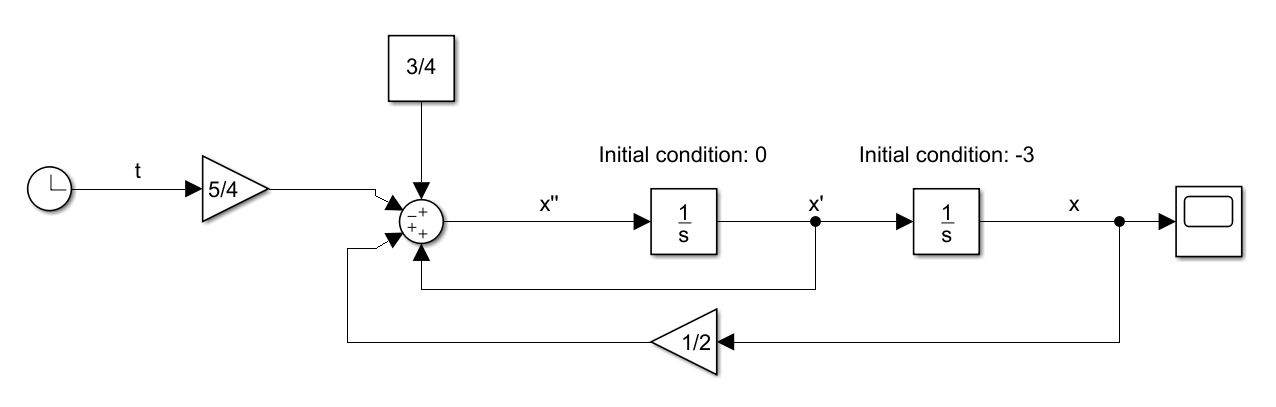
\includegraphics[width=0.9\textwidth]{images/schema2A_j.png}
        \caption{Simulink schema of the equation}
        \label{fig:simulink2}
    \end{figure}
    Initial conditions are 0 and -3 (from left to right).
    \begin{figure}[ht]
        \centering
        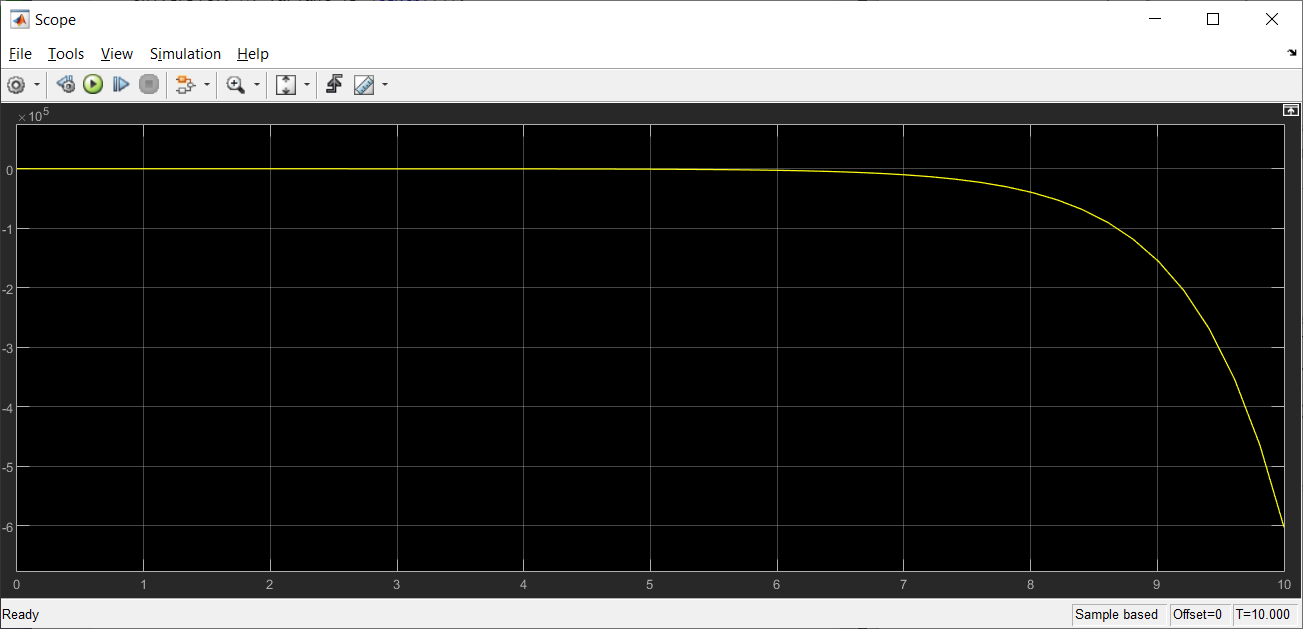
\includegraphics[width=0.9\textwidth]{images/plot2A_j.png}
        \caption{The plot of the solution}
        \label{fig:plot2a}
    \end{figure}
    
    \subsection{Simulink (with TF blocks)}
    
    \subsection{Matlab solution of the ODE}
    
    \lstinputlisting[caption=Solution of the ODE in Matlab, label={lst:listing1}, language=Matlab]{task2c_j.m}
    \begin{figure}[h]
        \centering
        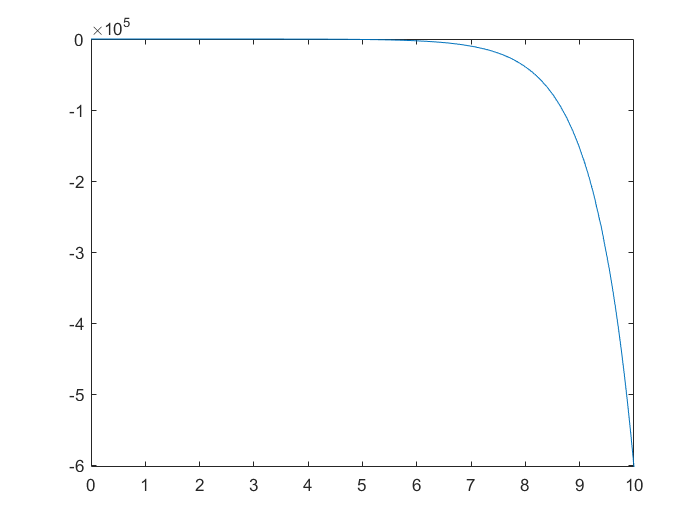
\includegraphics[width=0.9\textwidth]{images/solution2c_j.png}
        \caption{The plot of the Matlab solution}
        \label{fig:plot1c}
    \end{figure}
    
    \subsection{Laplace transform in Matlab}
    
    \lstinputlisting[caption=Solution of the ODE using Laplace transform in Matlab, label={lst:listing2}, language=Matlab]{task2d_j.m}
 
\section{ODE2SS (1)}
    Find the SS model of a system described by the following ODE:
    \begin{equation}
        x'' + 2x' - 3 = t + 5, \quad y = x'
    \end{equation}
    The SS model will look like
    \begin{align}
        \dot{x} &= Ax + Bu\\
        y &= Cx + Du
    \end{align}
    Let
    $x = \begin{bmatrix}
        x\\ 
        x'
    \end{bmatrix}$, 
    $u = \begin{bmatrix}
        1\\
        t
    \end{bmatrix}
    $. Let us express $x''$:
    \begin{equation}
        x'' = 0x - 2x' + t + 8
    \end{equation}
    Then 
    $A = \begin{bmatrix}
        0 & 1\\
        0 & -2
    \end{bmatrix}
    $ 
    and 
    $B = \begin{bmatrix}
        0 & 0\\
        8 & 1
    \end{bmatrix}
    $. It is easy to find matrices C and D. We are only interested in $x'$; thus, 
    $C = \begin{bmatrix}
        0 & 1
    \end{bmatrix}$
    and 
    $D = \begin{bmatrix}
        0 & 0
    \end{bmatrix}$.
    The final answer is:
    \begin{align}
        \dot{x} &=
        \begin{bmatrix}
            0 & 1\\
            0 & -2
        \end{bmatrix}
        x + 
        \begin{bmatrix}
            0 & 0\\
            8 & 1
        \end{bmatrix}
        u\\
        y &= 
        \begin{bmatrix}
            0 & 1
        \end{bmatrix}
        x + 
        \begin{bmatrix}
            0 & 0
        \end{bmatrix}
        u
    \end{align}
    
\section{ODE2SS (2)}
    Find the SS model of a system described by the following ODE:
    \begin{equation}
        x'''' + 3x''' + 4x'' + 2x' - 6 = 2u_1 + 2u_2, \quad y = x' + u_1 + u_2
    \end{equation}
    The SS model will look like
    \begin{align}
        \dot{x} &= Ax + Bu\\
        y &= Cx + Du
    \end{align}
    Let
    $x = \begin{bmatrix}
        x\\ 
        x'\\
        x''\\
        x'''
    \end{bmatrix}$, 
    $u = \begin{bmatrix}
        1\\
        u_1\\
        u_2\\
    \end{bmatrix}
    $. Then, obviously, 
    $\dot{x} = 
    \begin{bmatrix}
        x'\\ 
        x''\\
        x'''\\
        x''''
    \end{bmatrix}$. Let us express $x''''$:
    \begin{equation}
        x'''' = 0x - 2x' - 4x'' - 3x''' + 6 + 2u_1 + 2u_2
    \end{equation}
    Then
    \begin{align}
        A = 
        \begin{bmatrix}
            0 & 1 & 0 & 0\\
            0 & 0 & 1 & 0\\
            0 & 0 & 0 & 1\\
            0 & -2 & -4 & -3\\
        \end{bmatrix}, \quad 
        B = 
        \begin{bmatrix}
            0 & 0 & 0\\
            0 & 0 & 0\\
            0 & 0 & 0\\
            6 & 2 & 2\\
        \end{bmatrix}
    \end{align}
    and 
    \begin{equation}
        C = 
        \begin{bmatrix}
            0 & 1 & 0 & 0
        \end{bmatrix}, \quad
        D = 
        \begin{bmatrix}
            0 & 1 & 1
        \end{bmatrix}
    \end{equation}
    The final answer is:
    \begin{align}
        \dot{x} &=
        \begin{bmatrix}
            0 & 1 & 0 & 0\\
            0 & 0 & 1 & 0\\
            0 & 0 & 0 & 1\\
            0 & -2 & -4 & -3\\
        \end{bmatrix}
        x + 
        \begin{bmatrix}
            0 & 0 & 0\\
            0 & 0 & 0\\
            0 & 0 & 0\\
            6 & 2 & 2\\
        \end{bmatrix}
        u\\
        y &= 
        \begin{bmatrix}
            0 & 1 & 0 & 0
        \end{bmatrix}
        x + 
        \begin{bmatrix}
            0 & 1 & 1
        \end{bmatrix}
        u
    \end{align}
    
\section{ODE2SS (Python)}
    The code is available in the file "ode2ss.py".
    You need to have NumPy installed on your computer to run the script.
    
\end{document}